\documentclass{article}




% This format originated from that of NeurIPS 2023.
\usepackage[preprint,nonatbib]{neurips_2023}



\usepackage[utf8]{inputenc} % allow utf-8 input
\usepackage[T1]{fontenc}    % use 8-bit T1 fonts
\usepackage{url}            % simple URL typesetting
\usepackage{booktabs}       % professional-quality tables
\usepackage{amsfonts}       % blackboard math symbols
\usepackage{amsmath}       % blackboard math symbols
\usepackage{nicefrac}       % compact symbols for 1/2, etc.
\usepackage{microtype}      % microtypography
\usepackage{xcolor}         % colors
\usepackage{graphicx}
\usepackage{hyperref}       % hyperlinks
\usepackage[ruled,vlined]{algorithm2e}
\usepackage[style=authoryear,backend=bibtex]{biblatex}
\addbibresource{main.bib}

\newcommand{\B}[1]{\mathbf{#1}}
\newcommand{\TB}[1]{\textbf{#1}}
\newcommand{\etal}{\textit{et al}.~}
\newcommand{\robotConfig}{\mathcal{C}}


\title{A Survey of the Applications of Deep Reinforcement 
Learning for Motion Planning \& Control of Unmanned Aerial Vehicles}


% The \author macro works with any number of authors. There are two commands
% used to separate the names and addresses of multiple authors: \And and \AND.
%
% Using \And between authors leaves it to LaTeX to determine where to break the
% lines. Using \AND forces a line break at that point. So, if LaTeX puts 3 of 4
% authors names on the first line, and the last on the second line, try using
% \AND instead of \And before the third author name.


\author{%
  Baozhe Zhang \\
  School of Science and Engineering\\
  The Chinese University of Hong Kong, Shenzhen\\
  \texttt{baozhezhang@link.cuhk.edu.cn} \\
  % examples of more authors
  % \And
  % Coauthor \\
  % Affiliation \\
  % Address \\
  % \texttt{email} \\
  % \AND
  % Coauthor \\
  % Affiliation \\
  % Address \\
  % \texttt{email} \\
  % \And
  % Coauthor \\
  % Affiliation \\
  % Address \\
  % \texttt{email} \\
  % \And
  % Coauthor \\
  % Affiliation \\
  % Address \\
  % \texttt{email} \\
}


\begin{document}


\maketitle


\begin{abstract}
  TODO: Focus on the motion planning and control for quadrotors, 
  analyze 10 papers carefully
\end{abstract}


\section{Introduction}
Recently, micro aerial vehicles (MAVs) or 
unmanned Aerial Vehicles (UAVs), commonly known as drones, 
have emerged as a powerful tool in various industries, 
ranging from agriculture and real estate to filmography and delivery 
services. 
Their versatility and cost-effectiveness have led to a 
surge in applications that require multiple drones to operate 
collaboratively. 
Operating in real-world dynamic environments, 
these UAV systems need to navigate a wide range of 
challenges, 
including moving obstacles, inter-drone coordination, and 
real-time adaptability. 



The traditional planning and control pipelines for mobile robots' 
autonomous navigation have been extensively studied in recent
decades in the literature. 
Many complete systems with simultaneous localization 
and mapping (SLAM) and hierarchical 
planning and control frameworks can achieve outstanding 
autonomy.
For example, {\color{red} \textcite{zhou2019robust}} propose a robust and efficient 
quadrotor motion planning system for fast flight in 
three-dimensional complex environments.
{\color{red} \textcite{quan2023robust}} introduce a distributed motion planning 
trajectory optimization framework for large-scale quadrotor 
formation flight in dense environments.
Although traditional methods can achieve impressive performance, 
there are limitations and challenges associated with these methods: 
\begin{itemize}
  \item \TB{Complexity}. The hierarchical planning and control 
  methods consist of multiple layers of modules,   
  each of which requires fine-tuning of 
  its parameters, increasing the overall complexity of the system.
  \item \TB{Modeling Limitation}. Traditional methods rely on 
  accurate models of the environment and the system. However, 
  creating precise models, especially for complex systems like 
  drones, can be challenging. Small discrepancies between the 
  model and reality can lead to significant performance 
  degradation. 
  \item \TB{Generalizability}. Many traditional methods are 
  tailored to specific tasks, environments, 
  or robot platforms. Transferring them 
  to new tasks or settings often requires significant 
  modifications. 
\end{itemize}

The capability of the 
classical hierarchical motion planning framework is 
challenged 
as the complexity and randomness of robot application 
scenarios increase. 
Recent advancements in artificial intelligence have fostered 
the development of Deep Reinforcement Learning (DRL) - a branch 
of machine learning that trains agents to make sequential 
decisions by interacting with an environment. DRL has shown 
promise in addressing complex problems in robotics 
due to its ability to learn from large 
amounts of data and adapt to changes in real-time
\parencite{hwangbo2017control}.
DRL-based motion planning and control bring insights to 
overcome the challenges faced by traditional methods: 
\begin{itemize}
  \item \TB{Unified framework}. DRL allows for unified end-to-end 
  training and inference where planning and control can be 
  learned 
  jointly, potentially leading to more cohesive and optimal 
  solutions.
  \item \TB{Scalability with multiple agents}.  DRL can be 
  extended to multi-agent scenarios using techniques like 
  multi-agent reinforcement learning, enabling cooperative or 
  competitive behaviors among agents.
  \item \TB{Data-driven model}. Unlike model-based methods which 
  require precise system models, DRL can learn planning and  
  control policies directly from interaction data, potentially  
  avoiding modeling inaccuracies.
  \item \TB{Generalization}. Since many DRL methods are 
  model-free, the training can be generalized to different 
  robot platforms and even to many other tasks by changing 
  the reward functions defined in DRL algorithms.
\end{itemize}


Traditional motion planning and control methods have long 
provided 
reliable solutions in robotics. 
However, their limitation emerge with the increasing complexity of tasks, 
such as 
navigating in dynamic and stochastic environments.
In this survey, we try to demonstrate these challenges by providing 
a survey of the applications of DRL in the field 
of motion planning and control of UAVs.

\section{Traditional Motion Planning \& Control}

\begin{figure}[h]
  \centering
  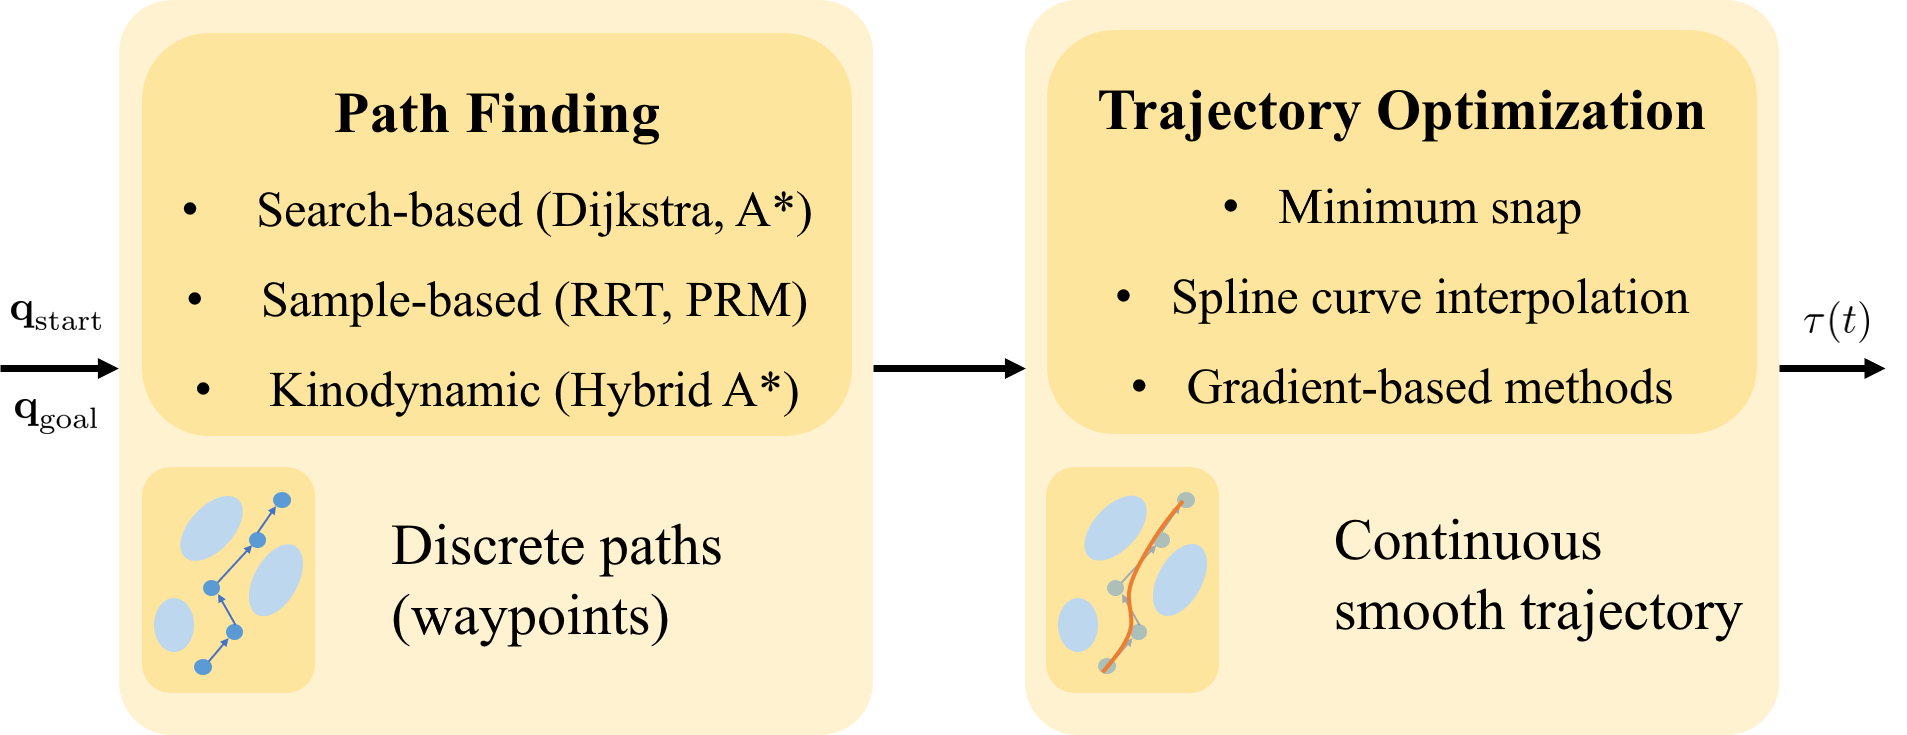
\includegraphics[width=.5\textwidth]{frontback.png}
  \caption{Hierarchical planning pipeline: The path-finding module 
finds a geometric collision-free path, and then trajectory
optimization module generates a continuous state-admissable and kinodynamically
feasible trajectory.}
  \label{fig:concept}
\end{figure}

Traditional planning and control frameworks are decoupled.
The path-planning (or motion-planning) module serves as a guide system 
for the low-level controller driving the robot's movement. 
This module needs to generate a geometrically 
collision-free and possibly kinodynamically feasible trajectory 
(or motion setpoints) for the low-level controller.
Then the low-level control module can use these motion 
setpoints to control the actuators on the robots to move.

The planning method usually consists of a hierarchical 
planning pipeline (Fig.~\ref{fig:concept}), a path-finding
and a trajectory-optimization module.
The path-finding problem is defined to 
find a path 
$
\tau : \left[0,1\right]\rightarrow \robotConfig_{\text{free}} 
$
such that  
$\tau(0) = \B{q}_{\text{start}} \in \robotConfig_{\text{free}}$ 
and
$\tau(1) = \B{q}_{\text{goal}} \in \robotConfig_{\text{free}}$, 
where $\robotConfig_\text{free}$ is the obstacle-free configuration space of the robot
\footnote{For UAVs, $\robotConfig_\text{free} \subset SE(3)$.}, 
and $\B{q}_{\text{start}}$ and $\B{q}_{\text{goal}}$ are the start and goal transformations, respectively.
The path $\tau$ can be a geometrically feasible discrete path.
To generate smooth trajectories with time profile 
for robots to 
follow based on discrete planned waypoints, the 
trajectory-optimization module is usually added to 
the pipeline. 
The control method aims to precisely command the 
UAV to track the given path (or trajectory), where 
general proportional-integral-derivative (PID) , 
robust, adaptive and optimal control methods may be utilized.


\section{Reinforcement Learning for Motion Planning \& Control}

In this section, we will discuss various RL algorithms for robotic 
motion planning and control, especially for UAV platforms. 
To ensure the coherency and consistency of the contents below, 
we adopt the following math representation: the states 
$\B{x}_t \in \boldsymbol{\mathcal{X}}$ 
and actions (inputs) $\B{u}_t \in \boldsymbol{\mathcal{U}}$ of a system (or an environment $\boldsymbol{\mathcal{E}}$) where $t\in\left[1,T\right]$ ($T$ may be $\infty$), 
the reward function $r(\B{x}_t, \B{u}_t)$, 
the initial state distribution $p(\B{x}_1)$, 
the transition probability $p(\B{x}_{t+1} | \B{x}_t, \B{u}_t)$, 
the policy $\pi(\B{u}_t | \B{x}_t)$, 
the return $G_t = \sum_{i=t}^T\gamma^{i-t}r(\B{x}_i, \B{u}_i)$ where $\gamma \in \left(0,1\right)$ is the discount factor, 
the value function $V(\B{x}_t) = \mathbb{E}\left[G_t | \B{x}_t\right]$, 
the action-value function $Q(\B{x}_t, \B{u}_t) = \mathbb{E}\left[G_t | \B{x}_t, \B{u}_t\right]$, 
and the goal is to maximize $G = \max \mathbb{E}\left[G_1 \right]$.

% Robot arm control has been a popular field for reinforcement learning 
% applications.
% \textcite{gu2017deep} propose an asynchronous off-policy update
% algorithm for DRL-based robotic manipulation, which utilizes
% the normalized advantage functions (NAF) proposed by 
% \textcite{gu2016continuous}.
% NAF parameterizes the advantage function into a quadratic form. 
% By introducing NAF, the Q function $Q(\B{x}_t, \B{u}_t)$ 
% in the continuous Q-learning can be represented in a way that
% the maximum, $\arg\max_{\B{u}_t}Q(\B{x}_t, \B{u}_t)$, can be determined 
% analytically during the Q-learning update.
% The Q function and the advantage function are represented as 
% \begin{equation}
% \label{eq:NAF}
% \begin{aligned}
%   Q(\B{x},\B{u}|\theta^Q) &= A(\B{x}, \B{u}|\theta^A) + V(\B{x}|\theta^V) \\
%   A(\B{x}, \B{u}|\theta^A) &=-\frac{1}{2} 
%   (\B{u} - \boldsymbol{\mu}(\B{x}|\theta^\mu))^\top
%   \B{P}(\B{x} | \theta^P)
%   (\B{u} - \boldsymbol{\mu}(\B{x}|\theta^\mu))
% \end{aligned}
% \end{equation}
% where $\theta^Q = \left\{ \theta^\mu, \theta^P, \theta^V \right\}$ is the 
% neural network parameters and $\B{P}(\B{x} | \theta^P)$ is a positive definite matrix.
% Therefore, $\arg\max_{\B{u}}Q(\B{x}, \B{u})$ is always given by
% $\boldsymbol{\mu}(\B{x} | \theta^\mu)$.
% In the robotic manipulation application, NAF is extended
% by asynchronous off-policy update using multiple threads (as in Algo.~\ref{algo:AsyncNAF})
% achieving better sample-efficacy.
% The asynchronous NAF algorithm is used to train a 7-DOF and the JACO arms 
% to perform tasks such as door pushing and pulling and pick and place.
% \begin{algorithm}[h]
%   \tcp{trainer thread}
%   Randomly initialize normalized Q network $Q(\B{x}, \B{u} | \theta^Q)$, where $\theta^Q = \left\{ \theta^\mu, \theta^P, \theta^V \right\}$\\
%   Initialize target network $Q^\prime$ with weight $\theta^{Q^\prime} \leftarrow \theta^Q$ \\
%   Initialize shared replay buffer $R \leftarrow \emptyset$ \\
%   \For{iteration=1,$I$} {
%     Sample a random minibatch of $m$ transitions from $R$ \\
%     Set 
%     $ y_i = 
%     \begin{cases}
%       r_i + \gamma V^\prime(x_i^\prime | \theta^{Q^\prime}) &\text{if}\quad t_i < T\\
%       r_i &\text{if}\quad t_i = T
%     \end{cases}
%     $\\
%     Update the weight $\theta^Q$ by minimizing the loss: 
%     $L = \frac{1}{m}\sum_i(y_i - Q(\B{x}_i, \B{u}_i))^2$ \\
%     Update the target network: 
%     $\theta^{Q^\prime} \leftarrow \tau \theta^{Q} + (1 - \tau)\theta^{Q^\prime}$
%   }
%   \tcp{collector thread $n,\;n=1,\dots,N$}
%   Randomly initialize policy network $\boldsymbol{\mu}(\B{x} | \theta_n^\mu)$ \\
%   \For{episode=1,$M$} {
%     Sync policy weight network $\theta_n^\mu \leftarrow \theta^\mu$ \\
%     Initialize a random process $\mathcal{N}$ for action exploration \\
%     Receive initial observation state $\B{x}_1 \sim p(x_1)$ \\
%     \For{t=1,T} {
%       Select action $\B{u}_t = \boldsymbol{\mu}(\B{x}_t | \theta_n^{\mu}) + \mathcal{N}_t$ \\
%       Execute $\B{u}_t$ and observe $r_t$ and $\B{x}_{t+1}$ \\
%       Send transition $(\B{x}_t, \B{u}_t, r_t, \B{x}_{t+1}, t)$ to $R$\\
%     }
%   }
%   \caption{Asynchronous NAF - N collector threads and 1 trainer thread}\label{algo:AsyncNAF}
% \end{algorithm}

Before diving into the recent work about RL in motion planning and 
control, we may first investigate this work proposed by 
\textcite{roy2002motion} on mobile robots.
In this early work, the motion planning method for the ground mobile robot 
generates a complete plan in the full state space of the robot, including orientation and velocity. 
It begins with an intermediate plan in a low-dimensional discrete space, using dynamic programming over a value function, and then projects this plan to the full state space. The plan is then refined through gradient ascent to increase the expected reward.
The state is defined as $\B{x}_t = \left[ x, y, \theta, v^t, v^r\right]^\top$ representing the $x$ and $y$ coordinates, orientation, linear 
and rotational velocities, respectively.
The action of this work is defined as $\B{u}_t = \left[ \Delta v^t, \Delta v^r \right]$.
The policy desired of this method is defined as a series 
of waypoints $\pi(\B{x}_i) = \left[ \B{w}_1, \dots, \B{w}_n\right]^\top$.
The value function in the matrix-vector form is defined as 
\[
  V(\pi_n) = \int_{t=0}^{T} G(\B{x}_t) R(\B{x}_t) dt 
           = \sum_{j=0}^{n-1} \int_{\B{x}(\B{w}_j)}^{\B{x}(\B{w}_{j+1})} G(\B{x}) R(\B{x}) dx 
\]
where $G(\cdot)$ is the state-transition matrix (this method
is model-based).
The algorithm for this method generating a series of waypoints is listed as follows:
\begin{algorithm}[h]
  \caption{Motion planning through policy search}
  \label{algo:roy2002}

  Use value iteration to run the dynamic program and extract a policy from 2-dimensional value function \\

  Determine the maximum likelihood trajectory and convert to a set of 5-dimensional waypoints to form the expected path. \\

  \While{$\neg$ converged}
  {
    \ForEach{Waypoint $\B{w}_j$}
    {
      Determine value contribution of trajectory from previous waypoint $\B{w}_{j-1}$ to next waypoint $\B{w}_{j+1}$ \\
      Measure gradient at endpoints \\
      Move waypoint $\B{w}_j$ along gradient until path segment value increases \\
    }

    Find lowest immediate reward along the trajectory \\
    Insert a new waypoint
  }
\end{algorithm}
This method, though a good attempt utilizing the core idea from RL to motion planning, 
is constrained by the complex definitions and framework, making
it not common and practical for quadrotor planning and control.
Besides, the generated waypoint-like path is not continuous nor 
kinodynamically feasible for high-speed vehicle such as quadrotors.

Control methods such as model prediction control (MPC) need
explicit and accurate state estimations of the robot.
RL can release the agent from the strict constraint and 
directly map the raw sensor data to control inputs to the agent.
In the work of \textcite{zhang2016learning}, the authors propose to combine MPC with RL in the framework of guided policy search, where MPC is used to generate data at training time, under full state observations provided by an instrumented training environment.
TODO: 


RL is utilized to directly control the quadrotor in \textcite{hwangbo2017control}.
This RL approach eliminates the need for predefined control structures, typically required in more traditional methods. 
Their new learning algorithm, which they claim is more suitable for quadrotor control than existing ones, is both conservative and stable for complex tasks. 
Their proposed approach is built on deterministic policy optimization using natural gradient descent.
TODO: 


\printbibliography

\end{document}